\chapter{State of the art short-term residential load forecasting techniques}
\label{cha:State of the art short-term residential load forecasting techniques}
Forecasting the electrical load of the different individual households has a couple of challenges. There should be dealt with the missing values, as discussed in section \ref{s:missing_data}. Also, the different time-series are influenced by exogenous factors as weather conditions and the day of the year. The dependency on exogenous variables can be a very non-linear relation and can have different effects on different households. For example depending on a house has solar panels, the consumption could be altered much. Only three indications of the temperature are given on a daily basis. Some additional information is know of certain households, but this data is very incomplete. Next, the individual load series have a high volatility and uncertainty with respect to a load signal on transmission level which shows more consistent seasonality and straight forward dependency on weather and calendar variables. This is because the contingency of the individual load data is mitigated due to averaging out of the uncertainty. Ofcourse, the obvious disadvantage is that only forecasts on this aggregated level can be made which is not the goal of our investigation.\\ To tackle the high non-linearity that is inherent to residential load forecasting in literature often ``Neural Networks'' to deal with this.

\section{Introduction to Neural Networks}
A  standard multilayer feedforward neuralnetwork with locally bounded piecewise continuous activation function can approximate any continuous function to any degree of accuracy if and only if the network's activation function is not a polynomial, as stated by \textbf{Leshno et al} in \textbf{1993}. This theorem proofs that a ``universal approximator'' exists for continuous functions, but it lacks the recipe to construct it. In \cite{Nielsen2015} it is shown that a feedforward network with a single layer is enough to approximate any function by a specified accuracy if the hidden layer has the possibility to add an unlimited amount of hidden neurons in its layer. It is discussed that when a function is discontinuous, which means that it makes sudden, sharps jumps, it is not possible to approximate the function by any prescribed accuracy. However, in practise a continuous approximation is often good enough.\\

Neural networks are suitable of learning very non-linear mappings between inputs and outputs. The difference between ``Deep Neural Networks'' and ``Shallow Neural Networks'' is the amount of layers of neurons are used inside the network. These layers of neurons, that are not inputs or outputs are called ``hidden neurons''. Because a ``Deep Neural Network'' has a a hierarchical layout of the different hidden layers, it not only learning features from the non-linear combinations of inputs, but uses other layers to learn features of combinations of features learned in lower hidden layers. This is possible because higher hidden layers get the outputs of lower hidden layers as input. As discussed in  \cite{Shi2018} due to this characteristic, deep learning is suitable to learn multiple uncertainties with differing sharing levels over different households e.g. the amount of sunshine. However, because of the higher expressiveness (and often the amount of the to learn parameters), a ``Deep Neural Network'' with respect to a ``Shallow Neural Network'', suffers more of overfitting as is discussed in section \ref{s:Problems}.

\subsection{MLP}
figure, activation function, equations

\subsection{CNN}

\subsection{RNN}

\subsection{Problems}\label{s:Problems}
Vanishing gradient problem --> short memory. Overfitting. Explosion of the gradient possible. tanh 
 ``Deep Recurrent Neural Network'' --> more parameters --> more overfitting


\textbf{Overfitting}\\
Early stopping --> can be seen as regularization
Training with regularization.
Dropout regularization 
Pruning

\textbf{Vanishing gradient}\\
LTSM --> vanishing gradient problem is not solved! Mittigated. 
GRU
Attention model
Transer model


\section{Short-Term residential electrical load forecasting}
%Things should get out of paper:
%Problem that was solved.
%Method
%Result
Classical ways to deal with uncertainty.\\


In this paper \cite{Shi2018} a novel pooling-based deep recurrent neural network is proposed which collects a group of customers load profiles into a pool of training inputs. Pooling of households historical loads to serve as input of the ``Deep Recurrent Neural Network'', is proposed to increase the data volume and diversity of load forecasting, which mitigates the effect of overfitting present in a DRNN. Also, due to the pooling of different households during training the DRNN is able to learn common uncertainties. From the pool of inputs every epoch a randomly chosen batch of load signals are fed to the network. LSTM is applied to mittigate the short term memory of the RNN. Additionally, there is been made use of early stopping to further avoid overfitting. To implement early stopping there has been looked at the ``MSE'' for k iterations, obtained by cross-validation. When the variance of this sequence gets smaller than a specified variable, training stops. When the training ends, performance is tested on each household by using the learned network to perform a feed-forward prediction of the electrical load.\\

An overview of the different steps that were done during the proposed method are: data cleaning and preprocessing $\rightarrow$ data pooling $\rightarrow$ data sampling $\rightarrow$ data training $\rightarrow$ benchmarking.\\

Performance of the proposed method was finally evaluated based on: 
\begin{enumerate}
	\item performance of the proposed method with respect to Vanilla RNN, SVR and DRNN (without pooling)
	\item the effect of the neural network depth and pooling
\end{enumerate}

The proposed DRNN with pooling outperforms all other four methods based on following three metrics:

\begin{equation}
	RMSE = \sqrt{\frac{\sum_{t=1}^{N}(\hat{y}_t-y_t)^2}{N}}
\end{equation}
\begin{equation}
	NRMSE = \frac{RMSE}{y_{max}-y_{min}}
\end{equation}
\begin{equation}
	MAE = \frac{\sum_{t=1}^{N}\abs{\hat{y}_t-y_t}}{N}
\end{equation}

The effect of the depth of the DRNN and the pooling method is depicted in Figure \ref{fig:Shi2018_result}. It can be seen that without the pooling method the DRNN only benefits from extra layers till three are used. This is because from that point, overfitting will reduce the generalization capacity of the DRNN. With the pooling technique, extra layers stays beneficial. It can thus be concluded that introducing extra hidden layers is a good choice to model the non-linear realations, but this can only be done efficiently when overfitting is mittigated by the use of a pooling strategy.The RNN with pooling used for benchmarking consisted out of five layers and thirty hidden units in each layer.

\begin{figure}[h!]
	\centering
	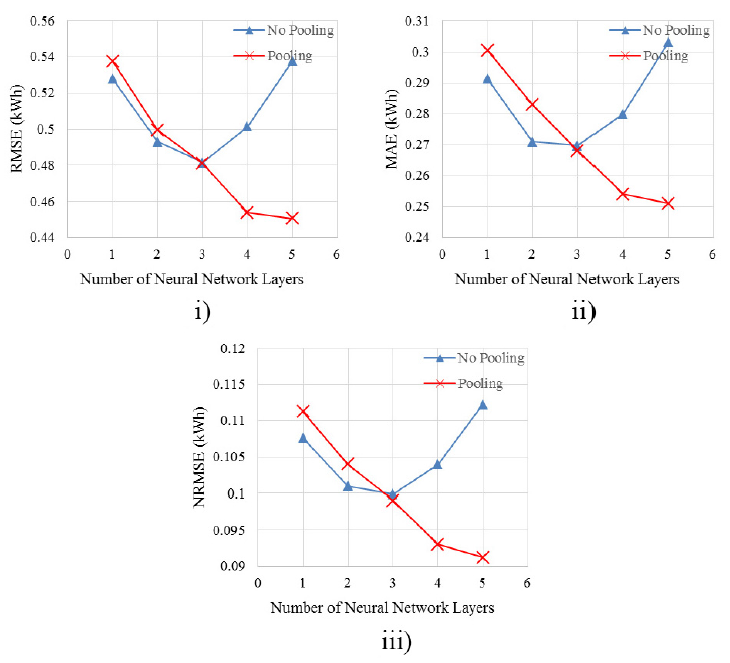
\includegraphics[width=1\textwidth]{Shi2018_result.png}
	\caption{Influence of the number of layers and the pooling method.}
	\label{fig:Shi2018_result}
\end{figure}














\section{Tables}
Tables are used to present data neatly arranged. A table is normally
not a spreadsheet! Compare \tref{tab:wrong} en \tref{tab:ok}: which table do
you prefer?

%\begin{table}
%  \centering
%  \begin{tabular}{||l|lr||} \hline
%    gnats     & gram      & \$13.65 \\ \cline{2-3}
%              & each      & .01 \\ \hline
%    gnu       & stuffed   & 92.50 \\ \cline{1-1} \cline{3-3}
%    emu       &           & 33.33 \\ \hline
%    armadillo & frozen    & 8.99 \\ \hline
%  \end{tabular}
%  \caption{A table with the wrong layout.}
%  \label{tab:wrong}
%\end{table}
%
%\begin{table}
%  \centering
%  \begin{tabular}{@{}llr@{}} \toprule
%    \multicolumn{2}{c}{Item} \\ \cmidrule(r){1-2}
%    Animal    & Description & Price (\$)\\ \midrule
%    Gnat      & per gram    & 13.65 \\
%              & each        & 0.01 \\
%    Gnu       & stuffed     & 92.50 \\
%    Emu       & stuffed     & 33.33 \\
%    Armadillo & frozen      & 8.99 \\ \bottomrule
%  \end{tabular}
%  \caption{A table with the correct layout.}
%  \label{tab:ok}
%\end{table}



\section{Conclusion}
The final section of the chapter gives an overview of the important results
of this chapter. This implies that the introductory chapter and the
concluding chapter don't need a conclusion.



%%% Local Variables: 
%%% mode: latex
%%% TeX-master: "thesis"
%%% End: 
